\subsection*{Problem A1}
\hfill \break
\begin{figure}[h!]
  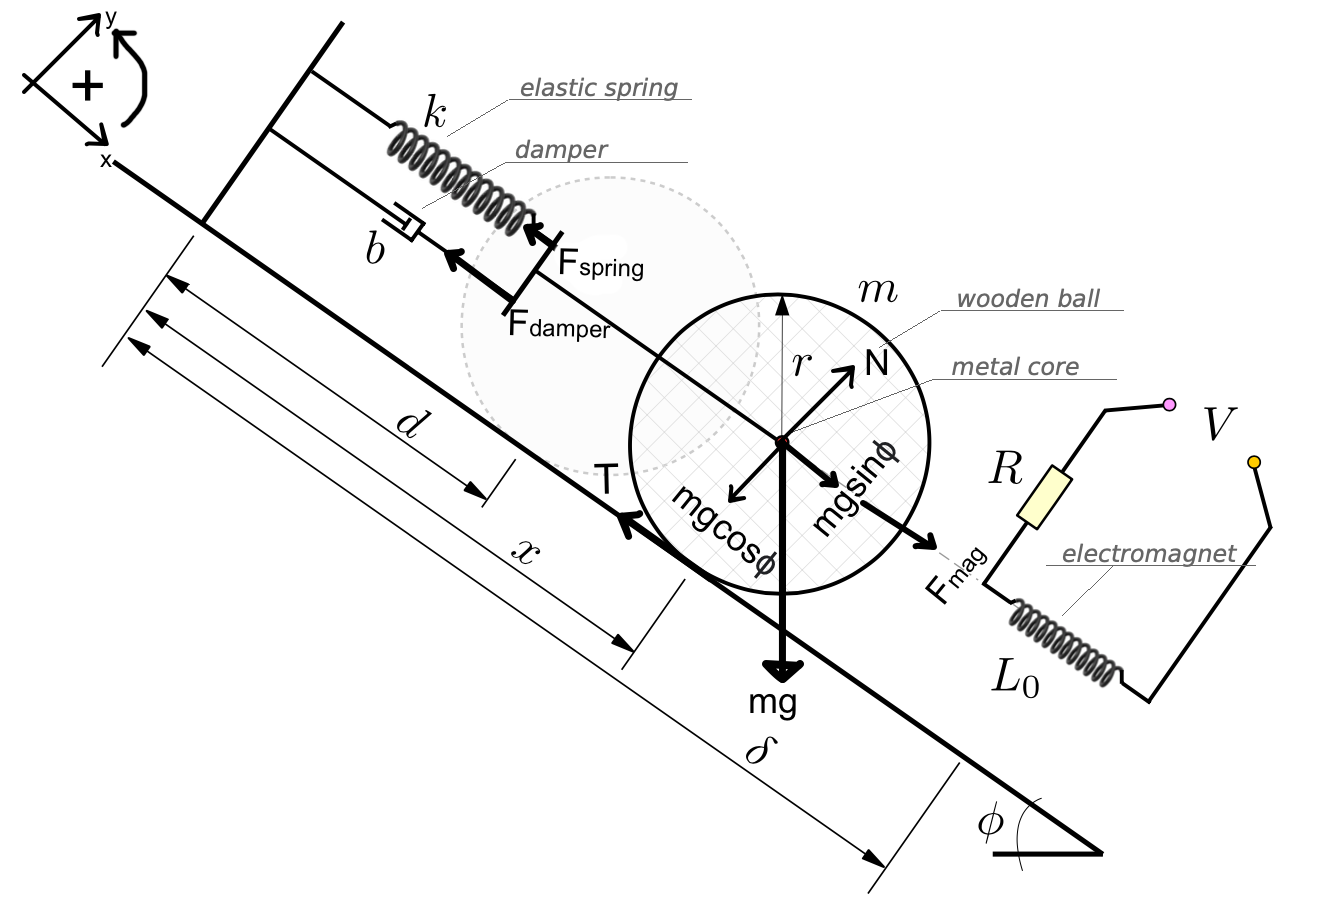
\includegraphics[width=0.7\textwidth]{Report/figures/main_diagram}
  \caption{System of a wooden ball on n inclined plane that can be attracted by an electromagnet, controlled by a voltage V, with forces applied labelled.}
  \label{fig:system}
\end{figure}

    \begin{align}
        F_{spring} &= k(x - d)\label{eq:3}\\
        F_{damper} &= b\dot{x}\label{eq:4}
    \end{align}
    \begin{equation} \label{eq:5}
        Tr &= -I\ddot{\theta} \therefore T = -\frac{I\ddot{\theta}}{r}
    \end{equation}
    \begin{align} 
        I &= \frac{2}{5} mr^2 \label{eq:6} \\
        \ddot{\theta} &= \frac{\ddot{x}}{r} \label{eq:7} \\\nonumber
    \end{align}
    Sub \eqref{eq:6} and \eqref{eq:7} into \eqref{eq:5}:
    \begin{equation} \label{eq:8}
        T = -\frac{2m\ddot{x}}{5}
    \end{equation}
    Apply Newtons 2nd Law of Motion to the system: 
    \begin{equation} \label{eq:9}
        F_{mag} + mg \sin{\phi} - T - F_{spring} - F_{damper} &= m \ddot{x}
    \end{equation}
    Sub \eqref{eq:2}, \eqref{eq:3}, \eqref{eq:4} and \eqref{eq:8} into \eqref{eq:9}:
    \begin{align} 
       \frac{cI^2}{y^2} + mg \sin{\phi} + \frac{2m \ddot{x}}{5} - k(x - d) - b \dot{x} &= m \ddot{x} \nonumber \\
       \text{(ODE)}\frac{cI^2}{(\delta - x)^2} + mg \sin{\phi} - k(x -d) - b \dot{x} &= \frac{3m}{5} \ddot{x}\label{eq:10}
    \end{align}
    Apply Kirchoff's Voltage Law to system circuit:
    \begin{align}
        V &= V_{R} + V_{L} \label{eq:11} \\
        V_{R} &= IR\label{eq:12}\\
        V_{L} &= L \dot{I}\label{eq:13}
    \end{align}
    Sub \eqref{eq:12}, \eqref{eq:13} into \eqref{eq:11}: 
    \begin{equation} \label{eq:14}
        V &= IR + L\dot{I}
    \end{equation}
    Sub \eqref{eq:1} into \eqref{eq:14}: 
    \begin{equation} \label{eq:15}
        \text{(ODE)}V &= IR + (L_0 + L_1 \exp{(-\alpha y)})\dot{I}
    \end{equation}
    \hfill \break
    Equations \eqref{eq:10} and \eqref{eq:15} are the ordinary differential equations for the system shown in Figure 1.
    
    
    
    